Spatial data and query processing have become ubiquitous due to proliferation of location-based services such as digital mapping, location-based social networking,
and geo-targeted advertising. Motivated by the performance benefits of learned indices
for one-dimensional data, this section explores the application of learned index for spatial data. The main motivation is to map spatial data into one-dimensional data through several steps and apply machine learning techniques to generate a learned index for the one-dimensional data.

\subsubsection{Motivation}

In the last section, we described a recursive model index (RMI) that consists of a number of machine learning models staged into a hierarchy to enable synthesis of specialised index structures, termed learned indexes. Provided with a search key $x$, RMI predicts the position of $x$'s data with some error bound, by learning the CDF over the key search space. However, as shown in Fig.  \ref{fig:Key_Distribution}, the idea of RMI is not applicable in the context of spatial data as spatial data invalidates the assumption required by RMI that the data is sorted by key and that any imprecision can be easily corrected by a localised search. Although it is possible to learn multi-dimensional CDFs, such CDFs will result in searching local regions qualified on one dimension but not all dimensions.

\begin{figure*}[t]
    \centering
    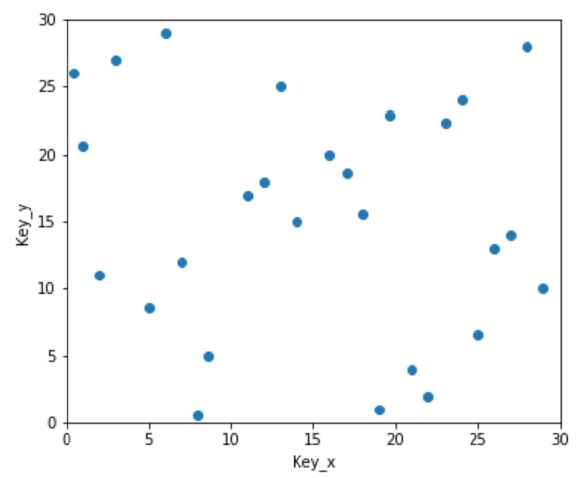
\includegraphics[width=0.6\textwidth]{graphs/Lisa_Key_distribution.png}
    \caption{Key Distribution in 2 dimensional case:Idea of learned indexes is not applicable in the context of spatial data as data is not sorted by key. Learning multidimensional CDFs will result in searching local regions qualified on one dimension but not all dimensions.}
    \label{fig:Key_Distribution}
\end{figure*}

\begin{mscexample}
For example, consider the joint cumulative function of two random variables X and Y defined as $F_{XY}(x, y)=P(X\leq x, Y\leq y)$.
The joint CDF satisfies the following properties:

\begin{itemize}
  \item  {$F_X(x)=F_{XY}(x,\infty)$, for any x (marginal CDF of X)}
  \item  {$F_Y(y)=F_{XY}(\infty,y)$, for any y (marginal CDF of Y)}
  \item  {if $X$ and $Y$ are independent, then $F_{XY}(x,y)=F_X(x)F_Y(y)$}
\end{itemize}

\end{mscexample}

\textcolor{blue} {Need to find a solid argument to explain why learning multi dimensional CDFs will result in  searching local regions qualified on one dimension. }

LISA solves this problem by partitioning search space into a series of grid cells based on the data distribution and building a\comment{partially monotonic} function map the data from $\mathbb{R}^d$ into $\mathbb{R}$, in our case, we have $d=2$. We call this function as \textit{Mapping Function}.
\subsubsection{Definitions}

This section presents the definition
\begin{enumerate}
	\item \textbf{Key}. A key k is a unique identifier for a data record with $k = (x_{0}, x_{1}) \in \mathbb{R}^{2}$. 
    %\textcolor{blue} {Need to check how to write d-1 in subscript }
    
	\item \textbf{Cell}. A grid cell is a rectangle whose lower and upper corners are points $(l_{0},l_{1}) and  (u_{0},u_{1})$, i.e.,  cell = $(l_{0},u_{0}) \times [l_{1},u_{1})$
	
	\item \textbf{Mapping Function}. A mapping function $\mathcal{M}$ is a function on the domain $\mathbb{R}^{2}$ to the non-negative range, i.e $M:[0,X_{0}]\times[0,X_{1}]\to [0,+\infty)$ such that $M(x_{0},x_{1}) \leq M(y_{0},y_{1})$ when $x_{0} \leq y_{0}$ and $x_{1} \leq y_{1}$.
	%TODO: add some example mapping functions
	
\end{enumerate}

\subsection{Baseline Method}  

We can extend the learned index method for range queries on spatial data by using a mapping function. This baseline method works as follows. We first sort all keys according to their mapped values and divide the mapped values into some cells such that each cell contains the same number of keys (except the last one). If a point $(x,y)$’s mapped value is larger than those of the keys stored in the first $i$ cells, i.e. $\mathcal{M}(x,y) > \sup \bigcup\limits_{j=0}^{i-1} M(C_{j})$, we store $(x,y)$ in the $(i+1)$th cell. 

For a range query, we have a query rectangle $qr = [l_{0},u_{0}) \times [l_{1},u_{1})$, we only need to predict the indices of $(l_{0}, l_{1})$ and $(u_{0},u_{1})$ namely $i_{1}$ and $i_{2}$ respectively. Then we scan the keys in $i_{2}-i_{1}+1$ cells, and find those keys that fall in the query rectangle qr. 

\begin{mscexample}
As shown in Fig. \ref{fig:BaseLine_Method_Limitation}, the key space is divided into 3 cells using the mapping function $\mathcal{M}((x,y))= x+y$. The query rectangle consisting of only $1$ key, falls inside the second part. During prediction, we need to find out the cells to which our query rectangle belongs (the $2^{nd}$ cell in our example). Once the cell is found, we need to compare the key of the query point, against all the possible keys in that cell until a match is found. This results in $8$ irrelevant points accessed for the range query that only contains one relevant key.
\end{mscexample}

\subsubsection{Training}

The training dataset for the baseline model can be notated as $(\boldsymbol{X}, Y)$ with entries notated as $(\boldsymbol{x},y)$. $\boldsymbol{X}$ represents the two dimensional key coordinates, and $Y$ represents the corresponding data item. 

In order to construct the baseline model, we need to have several parameters listed below:
\begin{enumerate}
	\item $N$, which represents the number of cells into which the key's mapped value space will be divided.
\end{enumerate}

As described in Algorithm \ref{Training_Lisa_Baseline}, during training, we perform the following operations:

\begin{enumerate}
	\item Sort all keys according to their mapped values.
	\item Divide the keys into equal sized cells
	\item Store the mapped values of first and last key for each cell into an array
\end{enumerate}



\begin{algorithm}[H]
    \SetAlgoLined
    \SetKwInOut{Input}{input}
    \SetKwInOut{Output}{Output}
    \Input{num\_of\_cells; trainset=[$(x,y);x \in \mathbb{R}^{2};y \in \mathbb{R}$]}
    \Output{M:Mapped Function}
     \For{$i\gets0$ \KwTo $len(x)$}{
            	\texttt{x[i].mapped\_value = x[i][0]+x[i][1]} \\
            
     }
     \texttt{Sort x based on x.mapped\_value}\\
     \texttt{Divide x into equal size pages according to num\_of\_cells}\\
     \texttt{Store mapped value of first and last key for each page }\\
      \For{$i\gets0$ \KwTo num\_of\_cells}
     {
         \texttt{denseArray[i].lower = first key in page i  } \\
		 \texttt{denseArray[i].upper = last key in page i  }
		
     }
     \caption{Training Algorithm for Lisa Baseline Method}
     \label{Training_Lisa_Baseline}
\end{algorithm}

For prediction, we find the cell corresponding to mapped value of the query point using binary search, scan this cell sequentially and compare the values of keys in the cell against the query point, until a match is found.

\subsubsection{Prediction}

\begin{algorithm}[H]
    \SetAlgoLined
    \SetKwInOut{Input}{input}
    \Input{\texttt{x\_test}: Key; \texttt{d:}the denseArray}
    \texttt{x\_test.mapped\_value = x\_test[0]+x\_test[1] } \\
    \For{$i\gets0$ \KwTo $len(denseArray)$}
    {
        \If{$\mathcal{M}(x\_test) \in [d[i].lower,d[i].upper]$} 
        {
		    \texttt{Key is in Page i } \\
		    \texttt{break }
		}
    }
  
 	 \texttt{Sequentially search for x\_test in page j} \\
     \caption{Prediction Algorithm for Lisa Baseline Model }
\end{algorithm}


\subsection{Lisa Overview}

%TODO: motivation 

Given a spatial dataset, we generate the mapping function $\mathcal{M}$, the shard prediction function $\mathcal{SP}$. Based on them, we build our index structure, LISA, to process range query and $K$NN query. LISA consists of four parts: the representation of grid cells, the mapping function $\mathcal{M}$, the shard prediction function $\mathcal{SP}$, and the local models for all shards. As illustrated in the Fig \ref{fig:Lisa_Framework}. the procedure of building LISA is composed of four parts.

\begin{figure*}[t]
    \centering
    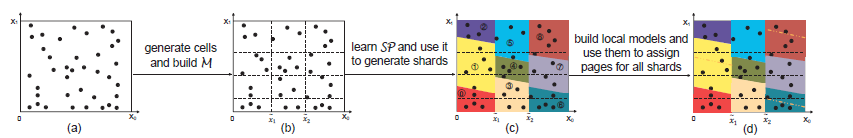
\includegraphics[width=17cm,height=4cm]{graphs/Lisa_Overview.png}
    \caption{Lisa Framework }
    \label{fig:Lisa_Framework}
\end{figure*}

\begin{enumerate}
	\item Grid cell partition.
	\item Mapping spatial coordinates into scalars, i.e. $\mathbb{R}^d\to\mathbb{R}$.
	\item Build shard prediction function $\mathcal{SP}$.
	\item Build local models.
\end{enumerate}

\subsubsection{Definitions}

This section presents the additional definition specific to Lisa implementation.

\begin{enumerate}
\setcounter{enumi}{3}
	\item \textbf{Shard}. The shard $S$ is the pre-image of an
interval $[a, b) \subseteq [0, +1)$ under the mapping function $\mathcal{M}$,  i.e., $S = M^{-1}([a.b))$. \\
%TODO: move this paragraph into somewhere more suitable
Given an initial data set, we divide the key space into cell grids based on the data distribution, map keys values to an one dimensional space using mapping function, followed by learning several monotonic shard prediction functions. After sorted, the one dimensional mapped value space is then divided into equal-length intervals, and one shard prediction function is learned for each interval, to partition the keys belonging to a particular interval, into different shards. As keys are sorted by mapped values before partitioning them into equal sized intervals, and all shards exhibit a total order with respect to their corresponding intervals in the mapped range(Shard Prediction function for each interval is monotonically increasing), following relationship holds \\
$ inf (M(S_{i}))  > sup (M(S_{j}))$ when $i > j$.

%TODO: claim that we will not work on the local models and tell the reason.
\item \textbf{Local Model}. Local model $L_{i}$ is a model
that processes operations within a shard $S_i$ . It keeps dynamic
structures such as the addresses of pages contained by $S_{i}$ .
\end{enumerate}

\subsection{Design and Implementation Details}
\subsubsection{Grid Cells Generation}
The first task in Lisa implementation is to partition the $2$ dimensional key space into a series of grid cells based on the data distribution along a sequence of axes. Then we number the cells along these axes as well. The principal idea behind this partition strategy is to divide the key space into cell boundaries and apply a mapping function to create monotonically increasing mapping values at the cell boundaries. 

%TODO: change the principal idea behind.

    $ M(x_{i} \in V) <  M(x_{j} \in V)$ when $i<j$, where $x_{i} \in C_{i}$ and $x_{j} \in C_{j}$ 
    
i.e. mapped value of a key in cell $i$ will always be less than mapped values of a key in cell $j$, if $i <j$.

\begin{mscexample}
	Consider the example shown in the figure \ref{fig:Cell_Parttion}: 27 keys are partitioned into $9$ cell, resulting in $3$ keys per cell. To partition the key space, we first sort the keys values according to $1^{st}$ dimension and divide the keys into $3$ vertical columns each containing $9$ keys. Then for each vertical column of $9$ keys, we sort the keys again according to $2^{nd}$ dimension, and divide the keys in each column into $3$ new cells. The number of cells $N$ into which the keys space is divided, is a hyper-parameter and found empirically using grid search.

\end{mscexample}

We need to sort the key space along the sequence of axis before we partition the keys value along that axis to make sure that cells don't contain overlapping keys. \\

\begin{figure*}[t]
    \centering
    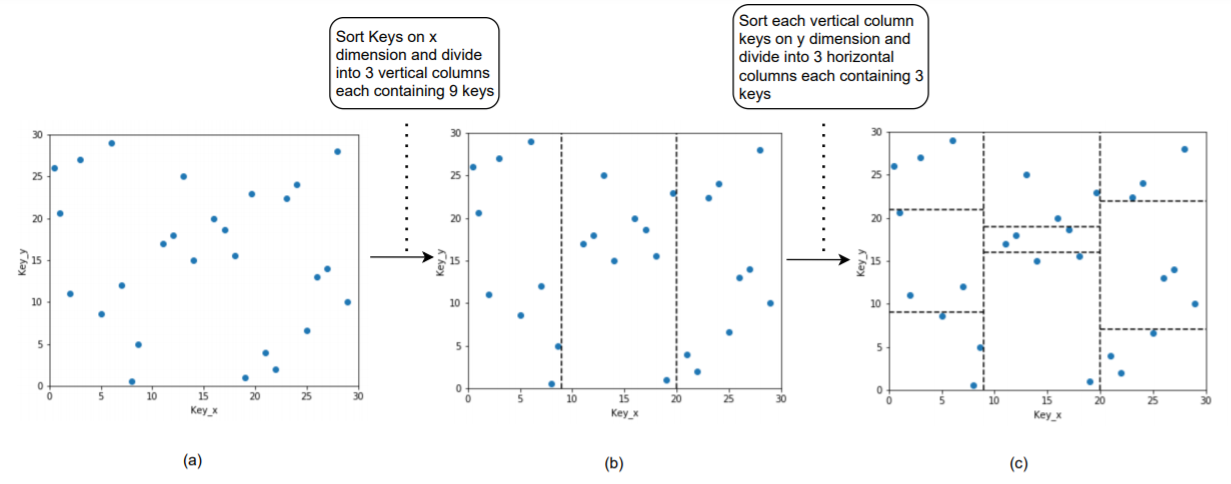
\includegraphics[width=1\textwidth]{graphs/Grid_Cell_Generation_Strategy_1.png}
    \caption{Cell Partition Strategy: \\
    1) : Sort Keys on x dimension and divide into 3 vertical columns each containing 9 keys\\
    2) : Sort each vertical column keys on y dimension and divide into 3 horizontal columns each containing 3 keys}
    \label{fig:Cell_Parttion}
\end{figure*}

\begin{algorithm}[H]
    \SetAlgoLined
    \SetKwInOut{Input}{input}
     \Input{\texttt{num\_of\_cells;x; y}}
     \texttt{trainset=[$(x,y);x \in \mathbb{R}^{2};y \in \mathbb{R}$]} \\
     \texttt{$keysPerPage =  len(x) / num\_of\_cells $}\\
     \texttt{Sort x based on first dimension x[:][0]]}\\
     \texttt{In first for loop, divide the keys into equal size subsets based on first dimension }\\
     \For{$i\gets0$ \KwTo $\sqrt(num\_of\_cells)$}  
     {
        \texttt{Store the 1st dimensional coordinates of first and last key for each cell. Each such cell will contain $keysPerPage*sqrt(num\_of\_cells)$ keys } \\
     }
     
     \texttt{Sort keys in each cell based on 2nd dimension,x[:][1] }\\
     
      \For{$i\gets0$ \KwTo $\sqrt{num\_of\_cells}$}
      {
         \For{$j\gets0$ \KwTo $\sqrt(num\_of\_cells)$}\
         {
            \texttt{Store the 2nd dimensional coordinates of first and last key for each cell.} \\
		 }
      }
     \caption{Grid Cell Generation Algorithm for Lisa Method}
     \label{Training_Lisa_Baseline}
\end{algorithm}

\subsubsection{Mapping Function}
A mapping function $\mathcal{M}$ is a function on the domain $\mathbb{R}^{2}$ to the non-negative range, i.e $M:[0,X_{0}]\times[0,X_{1}]\to [0,+\infty)$ such that
    $ M(x_{i} \in V) <  M(x_{j} \in V)$ if $i<j$, where $x_{i} \in C_{i}$ and $x_{j} \in C_{j}$. That means the mapped value of a key in cell $i$ will always be less than mapped values of a key in cell $j$, if $i <j$. 
    
Suppose $x = (x_{0}, x_{1})$ and $x \in C_{i} = [\theta^{(0)}_{i_0},\theta^{(0)}_{i_0+1}) \times [\theta^{(1)}_{i_1},\theta^{(1)}_{i_1+1}) $ then we define 
$$M(x) = i+ \frac {\mu(H_{i})}{\mu(C_{i})} $$ where $H_{i} = [\theta^{(0)}_{i_0},x_{0}) \times [\theta^{(1)}_{i_1},x_{1}) $ and $\mu$ is the Lebesgue measure on $\mathbb{R}^2$.

As shown in figure \ref{fig:Lebesgue_Measure}, in $2$-dimensional case, $\frac {\mu(H_{i})}{\mu(C_{i})}$ represents the fraction of the area covered by the key$(x_{0}, x_{1})$ to the total area of the cell. Since we are adding $i$, the index of the cell, to this fraction, the mapped value of a key in cell $i$ will always be less than mapped values of a key in cell $j$, if $i<j$. After calculating the mapped values of the data set, we sort the keys in each cell according to the mapped value. This results in the whole key space to be sorted according to the mapped value. Figure \ref{fig:Mapped_Cdf} shows the mapping of $2$ dimensional key space to one dimensional CDF.

\begin{figure*}[t]
    \centering
    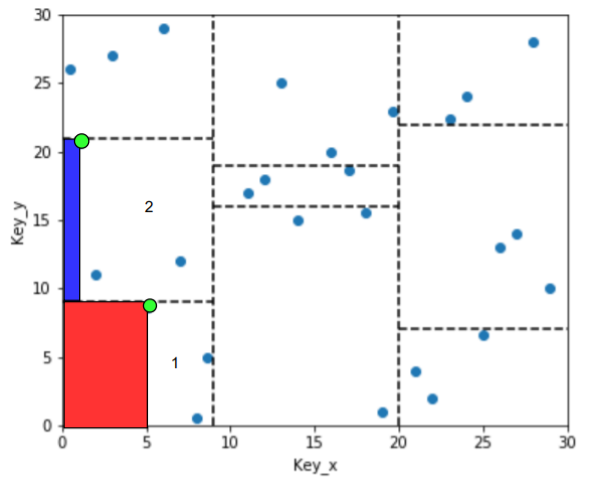
\includegraphics[width=0.6\textwidth]{graphs/Lebesgue_Measure.png}
    \caption{Lebesgue Measure Representation for 2 dimensional data\\
    1) Lebesgue Measure for the green point in first cell will be ratio of area of red rectangle divided by the total area of $1^{st}$ cell \\
    1) Lebesgue Measure for the green point in second cell will be ratio of area of blue rectangle divided by the total area of $2^{nd}$ cell}
    \label{fig:Lebesgue_Measure}
\end{figure*}

\begin{figure*}[t]
    \centering
    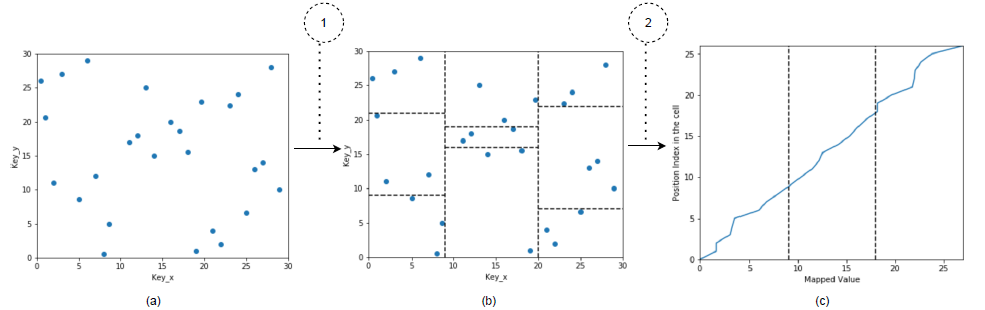
\includegraphics[width=1\textwidth]{graphs/Mapped_cdf.png}
    \caption{Mapping 2 dimensional key Values to one dimensional cdf\\
    1) Generate grid cells, and apply Lebesgue Measure to each cell.\\
    2) Sort key in each cell according to mapped value. Mapped values in consecutive cells are already sorted by mapping function definition. Plot the cdf of mapped values. }
    \label{fig:Mapped_Cdf}
\end{figure*}

\subsubsection{Shard Prediction Function}

After the mapping function, we get a dense array of mapped values. Then we partition them evenly into $U$ parts and let $\boldsymbol{M}_p=[m_1,\cdots, m_U]$. We train linear regression functions $\mathcal{F}_i$ on each interval and suppose $V+1$ is the number of mapped values that each $\mathcal{F}_i$ needs to process and $\Psi$ is the average number of keys falling in a shard. With these definitions, we know that each $\mathcal{F}_i$ generates $D=\ceil{\frac{V+1}{\Psi}}$ shards.

\begin{mscexample}
	For example, assume we have a dense array of mapped values as $$[1,1.2,2.2,3,3.4,4]$$ 
	
	We want to partition it into 2 parts, so we have $\boldsymbol{M}_p=[3]$ and $V+1=3$. In this case we will train $2$ linear regression functions. Suppose that the average number of keys in a shard is $\Psi=2$, then each $\mathcal{F}_i$ generates $D=\ceil{\frac{V+1}{\Psi}}=\ceil{\frac{3}{2}}=2$ shards.
\end{mscexample}


Then with a given $x$, the predicted shard is given by $\mathcal{SP}(x)=\mathcal{F}_i(x)+i\times D$, where $i=\text{binary-search}(\boldsymbol{M}_p,x)$. More specifically, we first determine $i$ by using binary search. The result tells which interval this $x$ should belong to. Then we find the corresponding linear regression function $\mathcal{F}_i$ and calculate $\mathcal{F}_i(x)$, which is the predicted shard.

\begin{mscexample}
	In the above example, given a key $x=2.2$, we first perform binary search in $\boldsymbol{M}_p$ and we found $i=1$. Then we find the first linear regression function $\mathcal{F}_1$ and calculate $\mathcal{F}_1(x)$. Since each linear regression function will yield $D=\ceil{\frac{V+1}{\Psi}}=2$ shards, the shards that the first linear regression function generates will be from $0$ to $1$ and the shards that the second linear regression function generates will be from $2$ to $3$. Hence, the predicted shard id is given by 
$$
\mathcal{SP}(x)=\mathcal{F}_i(x)+i\times D
$$
\end{mscexample}

Then the problem left is to train the linear regression functions $\mathcal{F}_i$. Let $\boldsymbol{x}=(x_0,\cdots,x_v)$ be the keys' mapped value that fall in $[m_{i-1}, m_i)$. Suppose that $\boldsymbol{x}$ is sorted, i.e. $x_i\leq x_j, \forall 0\leq i<j\leq v$. Let $\boldsymbol{y}=(0,\cdots, V)$. Then we build a piecewise linear regression function $f_i$ with inputs $\boldsymbol{x}$ and ground truth $\boldsymbol{y}$. For a given point with mapped value $m\in[m_{i-1}, m_i)$, its shard id is given by $\ceil{\frac{f_i(m)}{\Psi}}+i\times D$, i.e. $\mathcal{F}_i(x)=\frac{f_i(m)}{\Psi}$.

\begin{mscexample}
	In our previous example, in the interval $[0,3)$, we have $\boldsymbol{x}=(1,1.2,2.2)$ and $\boldsymbol{y}=(0,1,2)$. Then for a point with the mapped value $m=1.2$, the expected output will be $f_i(m)=1$ and the shard id is given by $\ceil{\frac{1}{2}}+0\times 2=1$. Hence, the point with mapped value $m=1.2$ will be allocated to the first shard. Then the problem is to train a continuous piecewise linear regression function in each interval. We constrain the piecewise linear regression function to be continuous so that it is guaranteed be monotonic.
\end{mscexample}

Formally, a piecewise linear function can be described as 

\begin{equation}
\label{piecewise_linear_function}
	f(x)= \begin{cases} 
      b_0+\alpha_0(x-\beta_0) & \beta_0\leq x < \beta_1 \\
      b_1+\alpha_1(x-\beta_1) &  \beta_1\leq x < \beta_2 \\
      \vdots \\
      b_\sigma+\alpha_\sigma(x-\beta_\sigma) &  \beta_\sigma\leq x \\
   \end{cases}
\end{equation}

In order to make this piecewise linear function continuous, the slopes and intercepts of each linear region depend on previous values. Formally, let $\bar{a}=b_0$, then Eq. (\ref{piecewise_linear_function}) reduces to

\begin{equation}
	\label{continuous_piecewise_linear_function}
	f(x)= \begin{cases} 
      \bar{\alpha}+\alpha_0(x-\beta_0) & \beta_0\leq x < \beta_1 \\
      \bar{\alpha}+\alpha_0(x-\beta_0) + \alpha_1(x-\beta_1) &  \beta_1\leq x < \beta_2 \\
      \cdots \\
      \bar{\alpha}+\alpha_0(x-\beta_0) + \alpha_1(x-\beta_1)+\cdots+\alpha_\sigma(x-\beta_\sigma) &  \beta_\sigma\leq x \\
   \end{cases}
\end{equation}


Then to make Eq. (\ref{continuous_piecewise_linear_function}) monotonically increasing, we only need to ensure that $$\sum_{i=0}^\eta \alpha_i\geq 0, \forall 0\leq \eta\leq \sigma$$

Let $\boldsymbol{\alpha}=(\bar{\alpha},\alpha_0,\cdots,\alpha_\sigma)$, the square loss function $L(\boldsymbol{\alpha},\boldsymbol{\beta})=\sum_{i=1}^{V}(f(x_i)-y_i)^2$. We then optimise $\boldsymbol{\alpha}$ and $\boldsymbol{\beta}$ iteratively.

Assume that $\boldsymbol{\beta}=\hat{\boldsymbol{\beta}}=(\hat{\beta_0},\hat{\beta_1},\cdots,\hat{\beta_\sigma})$ is fixed, then $\boldsymbol{\alpha}$ can be regarded as the least square solution of the linear equation $\boldsymbol{A\alpha}=\boldsymbol{y}$, where

$$
\boldsymbol{A}=\left[\begin{array}{ccccc}
1 & x_{0}-\hat{\beta}_{0} & \left(x_{0}-\hat{\beta}_{1}\right) 1_{x_{0} \geq \hat{\beta}_{1}} & \ldots & \left(x_{0}-\hat{\beta}_{\sigma}\right) 1_{x_{0} \geq \hat{\beta}_{\sigma}} \\
1 & x_{1}-\hat{\beta}_{0} & \left(x_{1}-\hat{\beta}_{1}\right) 1_{x_{1} \geq \hat{\beta}_{1}} & \ldots & \left(x_{1}-\hat{\beta}_{\sigma}\right) 1_{x_{1}} \geq \hat{\beta}_{\sigma} \\
\vdots & \vdots & \vdots & \ddots & \vdots \\
1 & x_{N}-\hat{\beta}_{0} & \left(x_{V}-\hat{\beta}_{1}\right) 1_{x_{V} \geq \hat{\beta}_{2}} & \cdots & \left(x_{V}-\hat{\beta}_{\sigma}\right) 1_{x_{V} \geq \hat{\beta}_{\sigma}}
\end{array}\right]$$

where $1_{x_{0} \geq \hat{\beta}_{1}}$ equals to $1$ if ${x_{0} \geq \hat{\beta}_{1}}$, otherwise it equals to $0$.

We have
\begin{equation}
 \begin{split}
	L(\boldsymbol{\alpha},\boldsymbol{\beta}) 
	 =(\boldsymbol{y-A\alpha})^T(\boldsymbol{y-A\alpha}) 
	&=\boldsymbol{y}^T\boldsymbol{y}-\boldsymbol{\alpha}{^T}\boldsymbol{A}^T\boldsymbol{y}-\boldsymbol{y}^T\boldsymbol{A\alpha}+\boldsymbol{\alpha}^T\boldsymbol{A}^T\boldsymbol{A\alpha} \\
	& = \boldsymbol{y}^T\boldsymbol{y}-2\boldsymbol{\alpha}^T\boldsymbol{A}^T\boldsymbol{y}+\boldsymbol{\alpha}^T\boldsymbol{A}^T\boldsymbol{A}\boldsymbol{\alpha}
\end{split}
\end{equation}

and if we let 

\begin{equation}
\label{alpha_form}
	\begin{split}
		\frac{\partial L(\boldsymbol{\alpha}, \boldsymbol{\beta})}{\boldsymbol{\alpha}}=2\boldsymbol{A}^T\boldsymbol{A}\boldsymbol{\alpha}-2\boldsymbol{A^T}\boldsymbol{y}=0 \\ \implies 
		\boldsymbol{\alpha}=(\boldsymbol{A}^T\boldsymbol{A})^{-1}\boldsymbol{A}\boldsymbol{y}
	\end{split}
\end{equation}


we get the $\boldsymbol{\alpha}$ with the given fixed $\boldsymbol{\beta}$. Clearly, different $\boldsymbol{\beta}$ give rise to different optimal parameters. Let $\boldsymbol{\alpha^\star}(\boldsymbol{\beta})$ be the optimal $\boldsymbol{\alpha}$ for a particular $\boldsymbol{\beta}$, then we want to find $\boldsymbol{\beta}$ such that


\begin{equation}
	L(\boldsymbol{\alpha^\star}(\boldsymbol{\beta^\star)}, \boldsymbol{\beta^\star})=\text{min}\{L(\boldsymbol{\alpha^\star}(\boldsymbol{\beta)}, \boldsymbol{\beta}) | \boldsymbol{\beta\in\mathbb{R}^{\sigma+1}}\}
\end{equation}

For $\boldsymbol{\beta}$, we define $\boldsymbol{r}=\boldsymbol{A\alpha-y}$ and 

$$
\boldsymbol{K}=\text{diag}(\bar{\alpha},\alpha_0, \cdots, \alpha_\sigma), \boldsymbol{G}=\begin{bmatrix}
 -1 & -1 & \cdots & -1 \\
  p_0^{(0)} & p_0^{(1)} & \cdots & p_0^{(V)} \\
  p_1^{(0)} & p_1^{(1)} & \cdots & p_1^{(V)} \\
  \vdots & \vdots & \ddots & \vdots \\
  p_\sigma^{(0)} & p_\sigma^{(1)}& \cdots & p_\sigma^{(V)} \\
\end{bmatrix}
$$

where $p_i^{(l)}=-1_{x_l\geq \beta_i}$. Then

$$
\boldsymbol{KG}=\begin{bmatrix}
 -\bar{\alpha} & -\bar{\alpha} & \cdots & -\bar{\alpha} \\
 0 & \alpha_0p_0^{(1)} & \cdots  & 0 \\
 \vdots & \vdots & \ddots & \vdots \\
 0 & 0 & \cdots & \alpha_\sigma p_\sigma^{(V)}
\end{bmatrix}
$$

then we have 

\begin{equation}
	g=\frac{\partial L(\boldsymbol{\alpha},\boldsymbol{\beta})}{\partial \boldsymbol{\beta}}=2\boldsymbol{KGr},
	Y=\frac{\partial g}{\partial \boldsymbol{\beta}}=2\boldsymbol{KGG}^T \boldsymbol{K}^T
\end{equation}
\textcolor{red}{Show how these are calculated}

As $g=\nabla_{\boldsymbol{\beta}} L$, $-g$ specifies the steepest descent direction of $\boldsymbol{\beta}$ for $L$. However, the convergence rate of $-g$ is low as it does not consider the second order derivative of $L$. Hence, we use Newton's method to perform the update along the direction of second derivative, $s=-\boldsymbol{Y}^{-1}g$. Newton's method assumes that the loss L is twice differentiable and uses the approximation with Hessian
The geometric interpretation of Newton's method is that at each iteration, it amounts to the fitting of a paraboloid to the surface of $L(\boldsymbol{\alpha},\boldsymbol{\beta})$  at the trial value $\beta_{k}$, having the same slopes and curvature as the surface at that point, and then proceeding to the maximum or minimum of that paraboloid. 
Hessian matrix, Y in our case is positive semidefinite and hence can be inverted. 
\begin{equation}
	Y=\frac{\partial g}{\partial \boldsymbol{\beta}}=2\boldsymbol{KGG}^T \boldsymbol{K}^T= 2 \boldsymbol{(KG)} (\boldsymbol{G}^T \boldsymbol{K}^T)=2 (\boldsymbol{G}^T \boldsymbol{K}^T)^T (\boldsymbol{G}^T \boldsymbol{K}^T)= 2\boldsymbol{({M}^TM)}
\end{equation}

\textcolor{red}{Show how these are calculated}
Y is a full rank matrix as columns of Y are linearly independent (all keys are independent of each other). To prove that Y is positive definite, we need to show that ${x}^TYx > 0,  \forall x \neq 0$. \\ 
${x}^TYx = {x}^T{M}^TMx = {(Mx)}^T(Mx) = \| Mx\|_{2}^{2} \geq 0,\forall x \neq 0 $

%\textcolor{red}{How to show that Y is positive definite and not just positive semidefnite.}  
%TODO: Show that Y is positive definite and explain why it matters

In the beginning, we set $\beta^{(0)}=x_0$ and $\beta_i^{(0)}=x_{\floor{i\times \frac{V}{\Psi}}}, \forall i\in[1,\sigma]$. Then we can obtain $\boldsymbol{\alpha}$ by solving Eq. (\ref{alpha_form}). Then at each step, we perform a grid search to find the step $lr^{(k)}$ such that the loss $L$ is minimal. Then at the next iteration, we increase $k$ by one and set 

$$
\boldsymbol{\beta}^{(k+1)}=\boldsymbol{\beta}^{(k)} + lr^{(k)}s^{(k)}
$$

%The iteration continues until $L$ converges, i.e. the $|L^{(k)}-L^{(k-1)}|<\delta$ where $\delta$ is a pre-set hyperparameter.

As described in Algorithm \ref{Shard_Training_Lisa}, we perform  following operations during shard training, :

\begin{enumerate}
	\item Divide the sorted mapped values into equal sized U intervals.
	\item Suppose V +1 is the number of mapped values in each interval and $\psi$ is the estimated average number of keys falling in a shard.
	\item For each interval, we want to build a monotonic regression
    model $ \mathcal {F}_{i}$ whose domain is $[m_{i-1},m_{i}]$ 
 
 	\item Each $\mathcal{F}_{i}$ generates D = $\ceil{\frac{V+1}{\Psi}}$ number of shards 
    
    \item $x =[x_0,\cdots, x_V] $ specifies the keys' mapped values in interval i, $[m_{i-1},m_{i}]$ 
    
    \item Given V +1 sorted mapped values $x =[x_0,\cdots, x_V]$ and their indices $y =[0,\cdots, V]$, each $\mathcal{F}_{i}$ is built and trained with the procedure mentioned in the algorithm \ref{Shard_Training_Lisa}.
    

\end{enumerate}

\begin{algorithm}[H]
    \SetAlgoLined
    \SetKwInOut{Input}{input}
    \Input{\texttt{$M_{p}$}, $\Psi$, U}
    \texttt{Partition $M_{p}$ into equal length U intervals $\boldsymbol{M}_p=[m_1,\cdots, m_U]$ }
    \For{$i\gets0$ \KwTo $U$}
    {   
        \texttt{$x =[x_0,\cdots, x_V] $ be the keys' mapped values
        in interval i} \\
        \texttt{$y =[0,\cdots, V]$ } \\
        \texttt{Initialize $\beta^{(0)}$ as $\beta^{(0)}=x_0$ and $\beta_i^{(0)}=x_{\floor{i\times \frac{V}{\Psi}}}, \forall i\in[1,\sigma]$} \\
        \While{\texttt{k} \textless \texttt{1000}} 
        {
            \texttt{Initialize $A^{(k)}$ according to \eqref{continuous_piecewise_linear_function}} \\
            \texttt{$\alpha^{(k)}= ((A^{(k)})^T A^{(k)})^{-1}(A^{(k)})^Ty$} \\
            
            \texttt{Calculate $g^{(k)}, Y^{(k)}$ } \\
            \texttt{$s^{k} = -(Y^{(k)})^{-1} g^{(k)}, $ } \\
            
            \texttt{Find update step $lr^{(k)}$ such that    L$(\alpha^\star(\beta^{k}+ lr^{(k)}s^{k}), \beta^{k}+ lr^{(k)}s^{k}) =\text{min}\{L(\alpha^\star(\beta^{k}+ lr^{(k)}s^{k}), \beta^{k}+ lr^{(k)}s^{k})\} $} \\
            
            \texttt{$\beta^{k+1} = \beta^{k}+ lr^{(k)}s^{k}$ } \\
        }
    }
    
    \caption{Shard Training Algorithm}
    \label{Shard_Training_Lisa}
\end{algorithm}

\subsubsection{Local Models for Shards}
Local models are not relevant to our implementation as all the data is contained in the memory.  

\subsubsection{KNN Query}
We do not know the analytical representation of shards, as we use machine learning model $ \mathcal{SP}$ to generate shards. Thus,it is difficult to apply traditional KNN query pruning strategies applicable for KD-Trees, to LISA model. 

Consider a query point $q_{knn}=x=(x_{0},x_{1})$, let $x^{'} \in V$ be the Kth nearest key to x in database at a distance value $\delta = \| x^{'}-x\|_{2} $. Lets define $ \mathcal{Q}(x,\delta) \triangleq [x_{0}-\delta, x_{0}+\delta) \times[x_{1}-\delta, x_{1}+\delta)$ and $\mathcal{B}(x, \delta)  \triangleq \{p \in V \mid \| x-p\|_{2} \leq \delta \} $.We can create a query rectangle $qr =  \mathcal{Q}(x, \delta + \epsilon)$ where $\epsilon \rightarrow 0$. As shown in Fig. \ref{fig:KNN_Query_Lisa}, K nearest keys to x are all in $\mathcal{B}(x, \delta)$ and thus in qr. KNN query can be solved using the range query if we can estimate an appropriate distance bound $\delta$ for every query point.

\begin{figure*}[t]
    \centering
    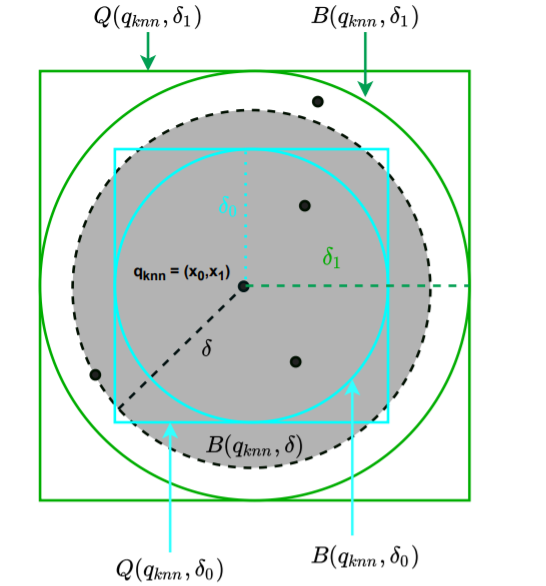
\includegraphics[width=0.7\textwidth]{graphs/KNN_Query_Lisa.png}
    \caption{KNN Query Implementation in Lisa(K=3)\\
    1)$q_{knn}$ represents the query point, $ \mathcal{Q}(x,\delta) \triangleq [x_{0}-\delta, x_{0}+\delta) \times[x_{1}-\delta, x_{1}+\delta)$, represents query rectangle and $ \mathcal{B}(x, \delta)$ represents the key space at distance $\delta$ containing K nearest keys.\\
    2)KNN query can be solved by range query if we can estimate an appropriate distance bound $\delta$ for every query point\\
    }
    \label{fig:KNN_Query_Lisa}
\end{figure*}








